%%%%%%%%%%%%%%%%%%%%%%%%%%% COORDINATESYSTEMS
% COORDSYS (ORIGOCOORDINATENAME, WIDTH, HEIGHT)
% Draws a Coordinatesystem around ORIGOCOORDINATENAME with a width of WIDTH and a height of HEIGHT, 
% names the beginning and end of axes, southwest corner, northwest corner, 
\newcommand{\ThreeDimCoordSys}[4]{
\coordinate (XY#1) at ([xshift=#2 cm, yshift=#3 cm]#1);
\coordinate (-XY#1) at ([xshift=-#2 cm, yshift=-#3 cm]#1);
\coordinate (X#1) at ([xshift=#2 cm]#1);
\coordinate (-X#1) at ([xshift=-#2 cm]#1);
\coordinate (Y#1) at ([yshift=#3 cm]#1);
\coordinate (-Y#1) at ([yshift=-#3 cm]#1);
%\path (#1); \pgfgetlastxy{\XCoord}{\YCoord}; % Extracting coordinates of the Origin
%\pgfmathsetmacro{\XCoordcm}{\XCoord/28.4527}
%\pgfmathsetmacro{\YCoordcm}{\YCoord/28.4527}
%\coordinate (Z#1) at (\XCoordcm, \YCoordcm,#4);
%\coordinate (-Z#1) at (\XCoordcm, \YCoordcm,-#4);
%\draw [help lines, step=.5cm] (-XY#1) grid (XY#1);
\coordinate (Z#1) at ([shift=(\ThirdAxisAngle : #4*\ThirdAxisUnit cm)]#1);
\coordinate (-Z#1) at ([shift=(\ThirdAxisAngle : #4*\ThirdAxisUnit cm)]#1);
\draw[->, name path=XAxis#1] (#1)--(X#1);
\draw[->, name path=YAxis#1] (#1)--(Y#1);
\draw[->, name path=ZAxis#1] (#1)--(Z#1);
}

% \DistanceLabel{SS}{AS}{-45}{1}{pos=.5}{1}
\newcommand{\DistanceLabel}[6]{
\coordinate(#1horgony) at ([shift=(#3:#4)] #1);
\coordinate(#2horgony) at ([shift=(#3:#4)] #2);
\draw[thin, red, <->] (#1horgony)--(#2horgony) node[#5]{#6};
\draw[opacity=.4, black] (#1)--(#1horgony);
\draw[opacity=.4, black] (#2)--(#2horgony);
}

%Lorentz(OriginalOriginCoord, ResultingOriginCoord, SpeedNum, PointCoord, Label)
% 
\newcommand{\Lorentz}[5]{
\path (#1); \pgfgetlastxy{\XCoord}{\YCoord}; % Extracting coordinates of the Origin
\pgfmathsetmacro{\XOrigin}{\XCoord} % Saving X coordinate
\pgfmathsetmacro{\YOrigin}{\YCoord} % Saving Y coordinate
\path (#4); \pgfgetlastxy{\XCoord}{\YCoord}; % Extracting coordinates of the Point
\pgfmathsetmacro{\XEvent}{\XCoord} % Saving X coordinate
\pgfmathsetmacro{\YEvent}{\YCoord} % Saving Y coordinate
\pgfmathsetmacro{\XEventWRTOrigin}{\XEvent-\XOrigin} % Relativizing to the origin
\pgfmathsetmacro{\YEventWRTOrigin}{\YEvent-\YOrigin} % Relativizing to the origin
\pgfmathparse{XLorentz(#3,\XEventWRTOrigin,\YEventWRTOrigin)} % transforming x
\pgfmathsetmacro{\XEventTr}{\pgfmathresult} % save the result of x
\pgfmathparse{YLorentz(#3,\XEventWRTOrigin,\YEventWRTOrigin)} % transforming y
\pgfmathsetmacro{\YEventTr}{\pgfmathresult} % save the result of y
\node[world](#5) at (
[xshift=\XEventTr pt,
 yshift=\YEventTr pt] #2){};
}

\usetikzlibrary{calc}
\usetikzlibrary{intersections}
\newdimen\XCoord
\newdimen\YCoord

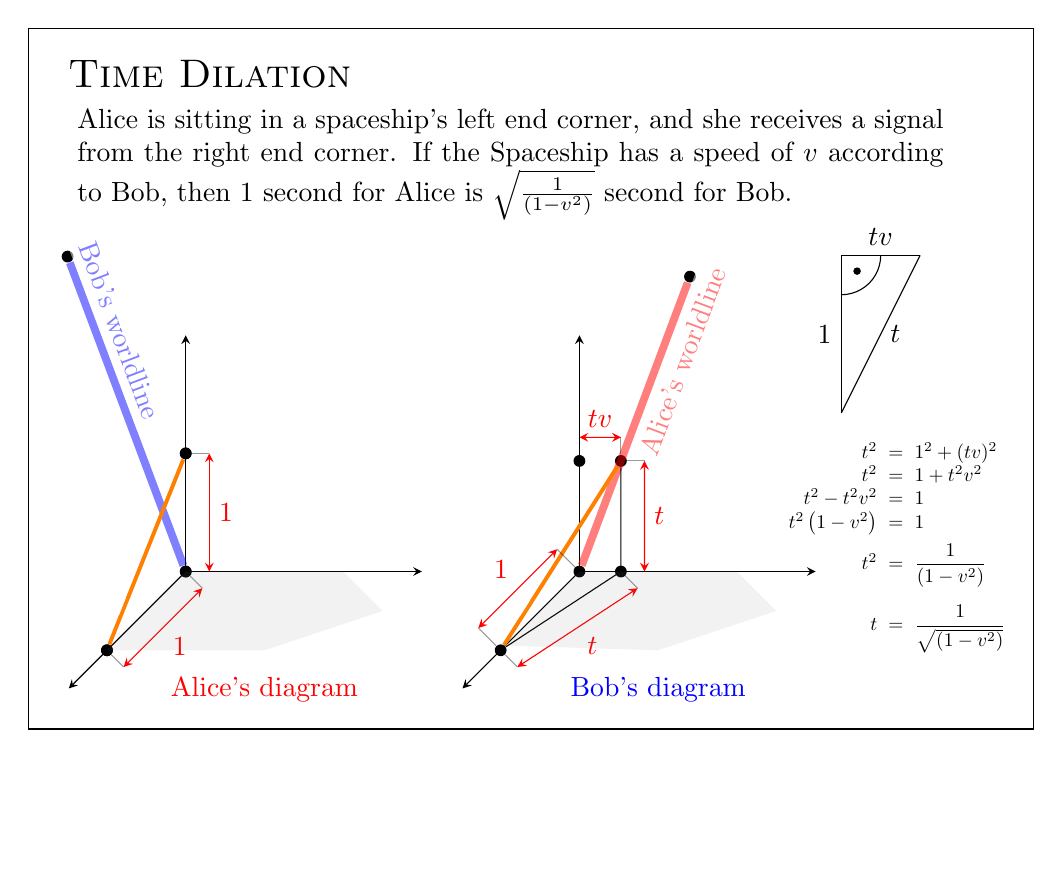
\begin{tikzpicture}[>=stealth, scale=1,
world/.style={inner sep=0, minimum size=.15cm, fill=black, circle},
worldline/.style={line width=1mm, rounded corners=1pt, opacity=.5},
axis/.style={->},
light/.style={orange, line width=.5mm},
]
\pgfmathdeclarefunction{XLorentz}{3}{\pgfmathparse{(#2 - #1*#3)/(sqrt(1-#1^2))}} % speed, spacecoord, timecoord
\pgfmathdeclarefunction{YLorentz}{3}{\pgfmathparse{(#3 - #1*#2)/(sqrt(1-#1^2))}} % speed, spacecoord, timecoord
\pgfmathsetmacro{\ThirdAxisAngle}{-135}
\pgfmathsetmacro{\ThirdAxisUnit}{.7}

%%%%%%%%%%%%%%%%%%%%%%%% DIA KEZDETE %%%%%%%%%%%%%%%%%%%%%%%%%%%

\node[anchor=north west, inner sep=0] at (0.5,8.5) {\textsc{\Large Time Dilation}}; %%%%%%% TITLE
%\node[anchor=north west, inner sep=0] at (0.5,8) {\textsc{\normalsize Role of Light}}; %%%%%%% SUBTITLE
\draw%[white]  %%%%%%%%%%%% SIZE OF THE SLIDE
      (0,0) rectangle (12.77,8.9);
%%%%%%%%% TEXT %%%%%%%%%%%%%
\node[anchor=north west] at (0.5,8) {\begin{minipage}{11cm}
Alice is sitting in a spaceship's left end corner, and she receives a 
signal from the right end corner. If the Spaceship has a speed of 
$v$ according to Bob, then 1 second for Alice is 
$\sqrt{\frac{1}{\left(1-v^2\right)}}$ second for Bob. 
\end{minipage}
};
%%%%%%%%%%%%%%%%%%%%%%%% KOORDINÁTARENDSZEREK %%%%%%%%%%%%%%%%%%%%%%%%%%%
\coordinate(O1) at (2,2) {} {};
  \ThreeDimCoordSys{O1}{3}{3}{3}
\coordinate(O2) at (7,2) {} {};
  \ThreeDimCoordSys{O2}{3}{3}{3}

%%%%%%%%%%
%% SETTINGS %%
%%%%%%%%%%

\coordinate (AliceStart) at (O1);
\coordinate (AliceEnd) at (2,6) {} {} {};
\coordinate (BobStart) at (O1); % Fontos hogy átmenjen az Origón, különben rossz a lorentz transzformáció!!
\coordinate (BobEnd) at (0.5,6) {} {} {};
\coordinate (SignalStart) at (1,1) {} {} {};
\coordinate (SignalBounced) at (2,3.5) {} {} {};

%%%%%%%%%%% Ezt lehetne macronak, speedszámítócuccnak
\path (BobStart); \pgfgetlastxy{\XCoord}{\YCoord}; % Extracting coordinates of the Origin
\pgfmathsetmacro{\XFirst}{\XCoord} % Saving X coordinate
\pgfmathsetmacro{\YFirst}{\YCoord} % Saving Y coordinate
\path (BobEnd); \pgfgetlastxy{\XCoord}{\YCoord}; % Extracting coordinates of the Point
\pgfmathsetmacro{\XSecond}{\XCoord} % Saving X coordinate
\pgfmathsetmacro{\YSecond}{\YCoord} % Saving Y coordinate
\pgfmathsetmacro{\SpeedBob}{(\XFirst-\XSecond)/(\YFirst-\YSecond)} % Relativizing to the origin
%%%%%%%%%%%%%%%%%%%%%%%%%%%%%%%%%%%

\Lorentz{O1}{O1}{0}{BobStart}{BS}
\Lorentz{O1}{O1}{0}{BobEnd}{BE}
\Lorentz{O1}{O1}{0}{SignalStart}{SS}
\Lorentz{O1}{O1}{0}{SignalBounced}{SB}
\Lorentz{O1}{O1}{0}{AliceStart}{AS}
%\Lorentz{O1}{O1}{0}{AliceEnd}{AE}
\Lorentz{O1}{O1}{0}{SignalStart}{SS}
\Lorentz{O1}{O1}{0}{SignalBounced}{SB}

\Lorentz{O1}{O2}{\SpeedBob}{AliceStart}{AS'}
\Lorentz{O1}{O2}{\SpeedBob}{AliceEnd}{AE'}
\Lorentz{O1}{O2}{0}{SignalStart}{SS'}
\Lorentz{O1}{O2}{\SpeedBob}{SignalBounced}{SB'}

\node[rotate=0, text=red, fill=white] at (3,0.5) {Alice's diagram};
\node[rotate=0, text=blue, fill=white] at (8,0.5) {Bob's diagram};
\draw[worldline, blue] (BS)--(BE) node[fill=white, sloped, above, pos=.75]{Bob's worldline};
\draw[worldline, red] (AS')--(AE') node[fill=white, sloped, below, pos=.75]{Alice's worldline};
\draw[light]  (SS)-- (SB) node[fill=white, sloped, above, pos=.2]{};
\draw[light]  (SS')-- (SB') node[fill=white, sloped, above, pos=.2]{};

%\pause %%%%%% PAUSE %%%%%%%%%%%
\DistanceLabel{SS}{AS}{-45}{3 mm}{pos=.5, below right}{1}
\DistanceLabel{AS}{SB}{0}{3 mm}{pos=.5, right}{1}
%\pause %%%%%% PAUSE %%%%%%%%%%%
\coordinate(r'SB') at ([yshift=-5cm]SB');
 \path[name path=Reflecting'SB'] (SB')--(r'SB');
\node[world,name intersections={of=XAxisO2 and Reflecting'SB', by=R'}] at (R'){};
\draw (R')--(SB');
\DistanceLabel{R'}{SB'}{0}{3 mm}{pos=.5, right}{$t$}
%\pause %%%%%% PAUSE %%%%%%%%%%%
\draw (R')--(SS');
\DistanceLabel{R'}{SS'}{-45}{3 mm}{pos=.5, below right}{$t$}
%\pause %%%%%% PAUSE %%%%%%%%%%%
 \coordinate(rSB') at ([xshift=-5cm]SB');
 \path[name path=ReflectingSB'] (SB')--(rSB');
\node[world,name intersections={of=YAxisO2 and ReflectingSB', by=R}] at (R){};
\DistanceLabel{R}{SB'}{90}{3 mm}{pos=.5, above}{$tv$}
%\DistanceLabel{O2}{R'}{90}{3 mm}{pos=.5, above, scale=.7, black}{$tv$}
%\pause %%%%%% PAUSE %%%%%%%%%%%
\DistanceLabel{O2}{SS'}{135}{4 mm}{pos=.5, above left}{$1$}

%\pause %%%%%% PAUSE %%%%%%%%%%%

\coordinate (v2) at (10.3264,6.0152) {} {};
\coordinate (v1) at (10.3264,4.0152) {} {};
\coordinate (v3) at (11.3264,6.0152) {} {};
\draw (v1)--(v2) node [midway, left]{$1$};
\draw (v2)--(v3) node [midway, above]{$tv$};
\draw (v3)--(v1) node [midway, right]{$t$};
\draw (10.8264,6.0152) arc (0.0009:-90.0055:0.5);
\draw[fill=black] ([xshift=  2mm, yshift= - 2mm]v2) circle (.4mm);
\node[anchor=north west, scale=.7] at (9.5,4) {\begin{minipage}{2cm}\[ \arraycolsep=1mm \begin{array}{rcl} 
    t^2 &=& 1^2 + (tv)^2
\\ t^2 &=& 1 + t^2v^2 
\\ t^2-t^2v^2&=&1
\\ t^2\left(1-v^2\right)&=&1
\\[1ex] t^2&=& \displaystyle  \frac{1}{\left(1-v^2\right)}
%\\[1.5em] t&=&\displaystyle \sqrt{\frac{1}{\left(1-v^2\right)}}
\\[1.5em] t&=&\displaystyle \frac{1}{\sqrt{\left(1-v^2\right)}}
\end{array}\]\end{minipage}};


\coordinate(Spaceship1) at (4,2) {};
\coordinate(Spaceship2) at (4.5,1.5) {};
\coordinate(Spaceship3) at (3,1) {};
\fill[fill opacity=.1, fill=gray]  (SignalStart) -- (O1) -- (Spaceship1) 
-- (Spaceship2) -- (Spaceship3)--cycle;

\coordinate(Spaceship1') at (9,2) {};
\coordinate(Spaceship2') at (9.5,1.5) {};
\coordinate(Spaceship3') at (8,1) {};
\fill[fill opacity=.1, fill=gray]  (SS') -- (O2) -- (Spaceship1') 
-- (Spaceship2') -- (Spaceship3')--cycle;

%\pgfmathsetmacro{\tee}{1/(sqrt(1-.87^2))}
%\node at (5,6) {E.g. $v= .87 \Rightarrow t= \tee$};
\end{tikzpicture}